% =====================================================================
% Clase -- Geometría 8° -- Trimestre I -- Semana 03
% Sesión 003 (mar 15 sep., 11:00, 50 min)
% Tema: Ángulos de un triángulo
% Subtema: Suma de ángulos internos y externos de un triángulo
% Hilo conductor del trimestre I: «Tales de Mileto y la medición de la gran pirámide»
% Tema 1 de la guía: Ángulos de un triángulo (tema:angulostriangulo)
% Material del docente (no se entrega a los estudiantes).
% =====================================================================
\documentclass[11pt]{article}
\makeatletter\def\input@path{{../../../../../plantillas/estilo/}}\makeatother
\usepackage{mmcantillo}
\guiadelestudiante{../../guia-didactica/guia-periodo-I-triangulos}

\tipodocumento{Clase}
\asignatura{Geometría}
\titulo{Semana 3: las leyes de los ángulos}
\grado{8°}
\periodo{I}

% DBA: PENDIENTE — la fila 003 de programacion.csv no tiene DBA, y la guía
% (decisión provisional 2 de su plan) tampoco le asigna uno. Propuesta, a confirmar
% por la docente: matematicas grado 8 · DBA 7 — Identifica regularidades y argumenta
% propiedades de figuras geométricas a partir de teoremas y las aplica en situaciones
% reales. Evidencias: «Describe teoremas y argumenta su validez a través de diferentes
% recursos (Software, tangram, papel, entre otros)» y «Resuelve problemas utilizando
% teoremas básicos».

\begin{document}

\encabezado*

\begin{center}
{\renewcommand{\arraystretch}{1.3}
\begin{tabularx}{\linewidth}{@{}l l l X l@{}}
  \toprule
  \textbf{Sesión} & \textbf{Fecha} & \textbf{Min} & \textbf{Subtema} & \textbf{Entregables}\\
  \midrule
  003 & mar 15 sep., 11:00 & 50 & Suma de ángulos internos y externos de un triángulo
      & Tarea (para el mar 22 sep.)\\
  \bottomrule
\end{tabularx}}
\end{center}

Esta sesión abre el Tema 1 de la guía y el hilo del trimestre: antes de medir la pirámide,
Tales quería saber \emph{por qué} se cumplen las propiedades de los triángulos. Se pasa de
comprobar con papel a demostrar con paralelas.
Referencia: \refguia{tema:angulostriangulo}.

\begin{nota}
\textbf{DBA pendiente.} La fila 003 no tiene DBA en \texttt{programacion.csv}. Se propone
el DBA 7 de grado 8 (evidencias «Describe teoremas y argumenta su validez\ldots{} papel» y
«Resuelve problemas utilizando teoremas básicos»); falta que la docente lo confirme.
\end{nota}

% ---------------------------------------------------------------------
\seccion{Sesión 003 — martes 15 de septiembre · 11:00 · 50 min}

\textbf{Objetivo.} Justificar que los ángulos internos de un triángulo suman $180^\circ$
(primero con papel, luego con una demostración con paralelas), y usar esa propiedad y la
del ángulo externo para calcular ángulos.

\textbf{Materiales.} Tablero; una hoja de papel y tijeras por pareja; regla; la guía del
estudiante.

\begin{center}
{\renewcommand{\arraystretch}{1.3}
\begin{tabularx}{\linewidth}{@{}l l X@{}}
  \toprule
  \textbf{Momento} & \textbf{Min} & \textbf{Actividad}\\
  \midrule
  Enganche & 0--5 & Leer el recuadro del hilo de la guía (Tales en Egipto). Repaso
    relámpago de la clasificación de las semanas 01--02: pedir un ejemplo de cada tipo por
    lados y por ángulos.\\
  Papel & 5--13 & Cada pareja dibuja un triángulo cualquiera (distinto al del vecino),
    marca sus tres ángulos, recorta las tres esquinas y las junta: forman un ángulo llano.
    Comparar entre parejas: pasa con todos. Pregunta: «¿esto \emph{demuestra} que siempre
    pasa?» (No: solo lo comprobamos con algunos triángulos, y el papel no es exacto.)\\
  Demostración & 13--23 & En el tablero, la figura de la guía: por $C$ se traza la
    paralela a $AB$; $\alpha'=\alpha$ y $\beta'=\beta$ por ser alternos internos; los tres
    ángulos en $C$ forman un llano. Enunciar el teorema. Consecuencias: a lo sumo un ángulo
    recto u obtuso; los agudos de un triángulo rectángulo son complementarios; ejemplo
    resuelto de la guía (ángulos de $30^\circ$, $60^\circ$ y $90^\circ$).\\
  Ángulo externo & 23--30 & Prolongar un lado y definir el ángulo externo. Deducirlo con
    el grupo: externo $+$ interno adyacente $=180^\circ$ y los tres internos suman
    $180^\circ$, luego el externo $=$ suma de los dos internos no adyacentes. Pregunta
    extra: ¿cuánto suman los tres externos? ($3\cdot180^\circ-180^\circ=360^\circ$.)\\
  Práctica guiada & 30--45 & Preguntas 1 a 4 del Tema 1 de la guía, en parejas; la
    docente pasa por los puestos y socializa la 2 (ángulo externo) y la 3 (argumentar).\\
  Cierre y tarea & 45--50 & Idea clave: \emph{lo que se comprueba con papel se demuestra
    con paralelas}. Asignar la tarea, para el martes 22 de septiembre.\\
  \bottomrule
\end{tabularx}}
\end{center}

\textbf{Figura para el ángulo externo (para copiar en el tablero).}

\begin{center}
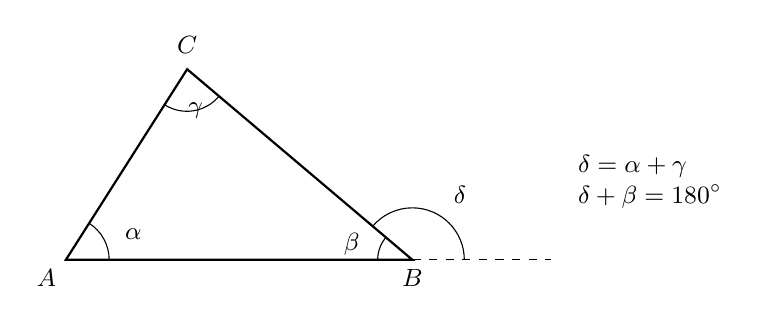
\begin{tikzpicture}[scale=1.1, every node/.style={font=\small}]
  \coordinate (A) at (0,0); \coordinate (B) at (4,0); \coordinate (C) at (1.4,2.2);
  \draw[thick] (A) -- (B) -- (C) -- cycle;
  \draw[dashed] (B) -- (5.6,0);
  \node[below left] at (A) {$A$}; \node[below] at (B) {$B$};
  \node[above=2pt] at (C) {$C$};
  \draw (0.5,0) arc (0:57.5:0.5); \node at (0.78,0.3) {$\alpha$};
  \draw (1.14,1.79) arc (237.5:319.8:0.48); \node at (1.5,1.72) {$\gamma$};
  \draw (3.6,0) arc (180:139.8:0.4); \node at (3.3,0.18) {$\beta$};
  \draw (4.6,0) arc (0:139.8:0.6); \node at (4.55,0.75) {$\delta$};
  \node[anchor=west, align=left] at (5.8,0.9) {$\delta = \alpha + \gamma$\\
    $\delta + \beta = 180^\circ$};
\end{tikzpicture}
\end{center}

\textbf{Respuestas de la práctica guiada} (preguntas del Tema 1 de la guía).
\begin{enumerate}
  % Ejercicio: triangulos-8-017
  \item $\frac{180^\circ - 50^\circ}{2} = 65^\circ$ cada uno.
  % Ejercicio: triangulos-8-021
  \item El externo es la suma de los internos no adyacentes: $110^\circ = 30^\circ + C$,
    así que $C = 80^\circ$ (y $B = 70^\circ$).
  % Ejercicio: triangulos-8-014
  \item Verdadera: dos ángulos obtusos sumarían más de $180^\circ$, y los tres ángulos de un
    triángulo suman exactamente $180^\circ$.
  % Ejercicio: triangulos-8-018
  \item $x + x + 2x = 180^\circ$, así que $x = 45^\circ$: miden $45^\circ$, $45^\circ$ y
    $90^\circ$.
\end{enumerate}

\begin{nota}
En la pregunta 3 no basta con «porque no se puede dibujar»: la respuesta tiene que usar la
suma de $180^\circ$. Es la primera vez del trimestre que se pide \emph{argumentar}; vale la
pena escribir en el tablero una respuesta modelo. Si sobra tiempo: la demostración con
paralelas es la de Euclides (\emph{Elementos} I.32).
\end{nota}

\end{document}
